\documentclass[12pt,a4paper]{article}

\usepackage[margin = 1.25 in ]{geometry}
\usepackage{graphicx} % Required for inserting images
\usepackage[english]{babel}
\usepackage[T1]{fontenc}
\usepackage{listings} % to print code
\usepackage{hyperref} % to manage hyperlink
\usepackage[acronym, toc]{glossaries} % to manage glossary
\usepackage[backend=biber, style=ieee]{biblatex} % Usage of IEEE style for References
\usepackage{titletoc} % Library to customize the Table of Content
\usepackage{csquotes}
\usepackage{booktabs} % For Tables
%\usepackage[firstpage]{draftwatermark}
%\SetWatermarkText{Draft}
%\SetWatermarkScale{5}

% Import References file
\addbibresource{references.bib}


\title{State of the Art\\Optimal scheduling for energy-harvesting batteryless sensory systems}
\author{Professors:\\Pierre-Yves Schobbens\\Laurent Schumacher\\Student: Quentin Franssen}
\date{11 March 2024}


% \dottedcontents{<section>}[<left>]{<above-code>}
% {<label width>}{<leader width>}
\dottedcontents{section}[0em]{\bfseries}{2.9em}{1pc}
\dottedcontents{subsection}[2em]{}{3.3em}{1pc}
%\dottedcontents{subsubsection}[4em]{}{3.3em}{1pc}

% center the toc heading
\renewcommand{\contentsname}{\centering Contents}


% Creating the glossary
\makeglossaries



\begin{document}

    % Load Glossary entries
    \newacronym{ipcc}{IPCC}{Intergovernmental Panel on Climate Change}
\newacronym{un}{UN}{United Nations}
\newacronym{sdg}{SDGs}{Sustainable Development Goals}
\newacronym{ep}{EP}{Environmental Performance}
\newacronym{ee}{EE}{Energy Efficiency}
\newacronym{et}{ET}{Emerging Technologies}
\newacronym{eh}{EH}{Energy Harvesting}
\newacronym{soc}{SoC}{System on Chip}
\newacronym{ml}{ML}{Machine Learning}
\newacronym{lpwan}{LPWAN}{Low-Power Wide-Area Network}
\newacronym{coap}{CoAP}{Constrained Application Protocol}
\newacronym{mqtt-sn}{MQTT-SN}{Message Queuing Telemetry Transport for Sensor Networks}

\newacronym{rfid}{RFiD}{Radio-frequency identification}
\newacronym{crfid}{CRFiD}{Computational Radio-frequency identification}
\newacronym{rom}{ROM}{Read-Only Memory}
\newacronym{ram}{RAM}{Read-Access Memory}
\newacronym{fram}{FRAM}{Ferroelectric Read-Access Memory}
\newacronym{eeprom}{EEPROM}{Electrically Erasable Programmable Read-Only Memory}
\newacronym{ciot}{CIoT}{Collaborative Internet of Things}
\newacronym{ar}{AR}{Activity Recognition}
\newacronym{ghm}{GHM}{Greenhouse Monitoring}
\newacronym{mems}{MEMS}{Micro-Electromechanical Systems}


\newglossaryentry{sustainability}{
  name={Sustainability},
  description={A holistic approach that considers environmental, social, and economic dimensions to meet present needs without compromising the ability of future generations to meet their own needs.\cite{unep_climatechangereport2023}}
}

\newglossaryentry{energyEfficiency}{
  name={Energy Efficiency},
  description={The goal to reduce the amount of energy required to provide products and services, by using less energy to achieve the same or an improved level of performance.}
}

\newglossaryentry{energyResilience}{
  name={Energy Resilience},
  description={The ability of energy systems to withstand, adapt to, and recover from disturbances while ensuring stable and reliable energy supply.\cite{unep_climatechangereport2023}}
}

\newglossaryentry{renewableenergy}
{
    name={Renewable Energy},
    description={Energy from sources that are naturally replenishing but flow-limited. Renewable resources are virtually inexhaustible in duration but limited in the amount of energy that is available per unit of time. These resources, such as sunlight, wind, rain, tides, waves, and geothermal heat, play a crucial role in sustainable energy systems and are central to reducing greenhouse gas emissions and combating climate change.\cite{unep_climatechangereport2023}}
}

\newglossaryentry{dpm}{
  name={DPM},
  description={Dynamic Power Management, a strategy for optimizing the power consumption of computing devices dynamically in response to workload demands and energy availability}
}

\newglossaryentry{lphd}{
  name={Low-Power Hardware Design},
  description={The design approach for creating hardware components that consume minimal power, essential for batteryless and energy-constrained devices}
}

\newglossaryentry{easd}{
  name={Energy-Aware Software Design},
  description={Software design methodology that prioritizes energy efficiency, aiming to reduce the energy consumption of software operations}
}

\newglossaryentry{ehi}{
  name={Energy Harvesting Integration},
  description={The incorporation of energy harvesting mechanisms into electronic systems, enabling them to capture and utilize ambient energy sources}
}

\newglossaryentry{ies}{
  name={Intermittent Energy Supply},
  description={Energy supply characterized by irregular availability, common with renewable energy sources like solar and wind}
}

\newglossaryentry{sopt}{
  name={Sensor Optimization},
  description={The process of enhancing sensor performance and efficiency, balancing accuracy, and resource consumption}
}

\newglossaryentry{adaptivealg}{
  name={Adaptive Algorithms},
  description={Algorithms that modify their operation or behavior in response to changes in their environment or input data}
}

\newglossaryentry{selflearningalg}{
  name={Self-Learning Algorithms},
  description={Algorithms capable of autonomously improving their performance over time through experience without explicit programming for all scenarios}
}

\newglossaryentry{ambientenergy}{
  name={Ambient Energy Sources},
  description={Environmental energy sources, such as solar, thermal, or kinetic energy, that can be harvested to power electronic devices}
}

\newglossaryentry{energyharvesting}{
  name={Energy Harvesting},
  description={The process of capturing energy from ambient sources and converting it into usable electrical power}
}

\newglossaryentry{pmc}{
  name={Power Management Circuit},
  description={Circuits designed to manage and optimize the power usage of electronic devices, crucial for energy efficiency}
}

\newglossaryentry{ulpc}{
  name={Ultra-Low-Power Components},
  description={Electronic components engineered to operate with extremely low power consumption, suitable for energy-harvesting applications}
}

\newglossaryentry{est}{
  name={Energy Storage Technologies},
  description={Technologies used for the storage of energy, such as batteries and \gls{supercap}, particularly important for managing intermittent energy supplies}
}

\newglossaryentry{supercap}{
  name={Supercapacitor},
  description={A high-capacity capacitor with capacitance values much higher than other capacitors but lower voltage limits, which bridges the gap between electrolytic capacitors and rechargeable batteries. It stores energy through a static mechanism, which allows for rapid charging and discharging cycles compared to batteries}
}

\newglossaryentry{poweraware}{
  name={Power Aware},
  description={Refers to the system's capability to monitor and adapt its power consumption in real-time, aiming to optimize power usage and performance without compromising the operational needs of the system.}
}

\newglossaryentry{energyaware}{
  name={Energy Aware},
  description={Involves understanding and managing the overall energy consumption of a system over a period, focusing on achieving long-term energy efficiency and sustainability by optimizing energy usage patterns and behaviors.}
}

\newglossaryentry{process}{
  name={Process},
  description={In computing, a process is an instance of a computer program that is being executed. It contains the program code and its current activity.}
}

\newglossaryentry{eveh}{
    name={EVEH},
    description={The Electromagnetic Vibration Energy Harvesters, or EVEH, were proposed in the late 1900s. These transducers transform kinetic energy (vibration) into electrical energy.}
} 

\newglossaryentry{task}{
  name={Tasks},
  description={Tasks can be considered as smaller than \gls{process}, more specific units of work executed by the computer.}
}

\newglossaryentry{fsm}{
  name={Finite State Machines (FSM)},
  description={are computational models used to design logic in systems. They transition from one state to another based on certain inputs and a set of rules. FSMs are particularly useful in ultra-low power, battery-less IoT devices because they can efficiently manage device operations with minimal power usage. By simplifying the control logic into defined states, FSMs can help reduce the power consumed by these devices during both active and idle periods.}
}

\newglossaryentry{electrostatic}{
    name={Electrostatic},
    description={Electrostatic phenomena involve the interactions and forces between stationary electric charges, explained by Coulomb's law, which includes the forces that electric charges exert on each other without moving.}
}

\newglossaryentry{piezoelectric}{
    name={Piezoelectric},
    description={It generally refers to the ability of certain materials to generate an electric charge in response to applied mechanical stress. This effect is reversible, meaning that these materials can also change shape when an electric field is applied, a phenomenon used in various applications such as sensors, actuators, and generators\cite{enwiki:1212461326}.}
}

\newglossaryentry{electromagnetic}{
    name={Electromagnetic},
    description={It encompasses the laws and phenomena associated with the electromagnetic force, which is a fundamental interaction between particles with electric charges. The electromagnetic force is responsible for practically all the phenomena encountered in daily life (with the exception of gravity), including the technologies we use, from household appliances to understanding the structure of atoms\cite{enwiki:1210790681}.}
}

\newglossaryentry{magnetorestrictive}{
    name={MagnetoRestrictive},
    description={Similar to piezoelectric materials, magnetostrictive materials change their shape or dimensions in the presence of a magnetic field. This property is utilized in various applications such as sensors and actuators, where the conversion between magnetic and mechanical energy is required. While a direct source definition was not retrieved in this search, this explanation aligns with the known scientific understanding of the term.}
}






\newglossaryentry{rehash}{
    name={REHASH},
    description={is a framework, is a flexible heuristic-adaptation-based runtime for intermittently-powered devices.\cite{gitlab:rehash}},
    first={REHASH}
}

\newglossaryentry{mnist}{
    name={MNIST},
    description={is a framework, is a flexible heuristic-adaptation-based runtime for intermittently-powered devices.\cite{gitlab:rehash}},
    first={MNIST}
}

\newglossaryentry{heuristic}{
    name={Heuristic},
    description={is a function developed-defined logic statement that takes an equation composed of measured signals and calculates a binary outcome, i.e. adapt up, or adapt down. The outcome of the heuristic function decides when to adapt tasks and knobs},
    first={Heuristic}
}


\newglossaryentry{allornothingsemantics}{
    name={All-Or-Nothing semantics},
    description={refers to a principle or approach where an action is executed in its entirety or not at all. In other words, if any part of the action fails or encounters an issue, the entire action is considered unsuccessful, and no changes are made to the system. This ensures that data remains in a consistent state and prevents partial changes that could lead to inconsistencies or errors. e.g: Transaction on Database},
    first={All-Or-Nothing semantics}
}

\newglossaryentry{atomizeprocesses}{
    name={Atomizing processes},
    description={is the application of the \textit{Divide and Conquer} principle at a lower level. In this approach, tasks are broken down into subtasks that remain indivisible. If one of these subtasks fails, the entire process becomes stuck until that specific action succeeds. This ensures that the process maintains its integrity and consistency throughout its execution.\cite{enwiki:1165389216}},
    first={Atomizing processes}
}

\newglossaryentry{nonVolatileMemory}{
    name={Non-Volatile Memory},
    description={is a type of memory where \textbf{data persists even in the absence of power}. Examples of NVM include \gls{rom}, flash drives, \gls{fram}, \gls{eeprom} and other storage devices.},
    first={Non-Volatile Memory}
}

\newglossaryentry{volatileMemory}{
    name={volatileMemory},
    description={yis a type of memory utilized for current tasks within a running session. This form of memory offers faster data access but is temporary in nature, as data is \textbf{lost once power is disconnected}. \gls{ram} is a prime example.},
    first={Volatile Memory}
}

\newglossaryentry{fault tolerance}{
    name={fault tolerance},
    description={The ability of a system to continue operating without interruption when one or more of its components fail}
}

\newglossaryentry{cryptographic algorithms}{
    name={cryptographic algorithms},
    description={Mathematical algorithms used to secure data against unauthorized access or modification}
}

\newglossaryentry{blockchain}{
    name={blockchain},
    description={A distributed database that is used to maintain a continuously growing list of records, called blocks, which are linked and secured using cryptography}
}

\newglossaryentry{electronic waste}{
    name={electronic waste},
    description={Discarded electrical or electronic devices. Used electronics which are destined for reuse, resale, salvage, recycling, or disposal are also considered electronic waste}
}


%\newacronym{iot}{IoT}{Internet of Things}

\newglossaryentry{iot}
{
    name={Internet of Things (IoT)},
    description={concept involves devices equipped with sensor(s) that are connected to a network, enabling the digitalization of the physical world through continuous monitoring. \cite{IoT_Definition}},
    first={Internet of Things (IoT)}
}


\newglossaryentry{batteryless}
{
    name={Batteryless},
    description={is a device is one that can operate without a battery, relying instead on energy spikes to charge its capacitor to activate. This process enables the device to wake up and operate for a brief period, typically a few milliseconds.},
    first={batteryless}
}


\newglossaryentry{terraswam}{
    name={TerraSwarm},
    description={TerraSwarm is a research initiative that focuses on developing technologies related to smart dust and the \gls{iot}. It aims to create a "swarm" of smart devices that can sense and interact with the physical world in real-time. The term "terra" in TerraSwarm represents the connection to the Earth's environment. TerraSwarm's research encompasses various areas such as system architecture, energy efficiency, security, and scalability to enable the deployment of large-scale networks of interconnected smart devices. This project is ended from the 31 December 2017\cite{terraSwamWebsite}.}
}

\newglossaryentry{smartdust}{
    name={Smart Dust},
    description={referes to tiny, autonomous wireless sensors that are about the size of a grain of dust. These sensors are equipped with processing, communication, and environmental sensing capabilities, such as temperature, humidity, light sensors, and more. They are designed to be deployed in the environment to monitor and collect data on various phenomena. These sensors are typically interconnected in ad hoc networks, allowing them to communicate with each other and transmit the collected data to base stations or other devices for analysis. The idea behind Smart Dust is to create a large-scale network of distributed sensors that can be used for monitoring extensive areas, such as industrial environments, urban areas, natural habitats, etc\cite{smartDust}.}
}

\newglossaryentry{photovoltaic}{
    name={Photovoltaic},
    description={refers to the conversion of light into electricity using semiconducting materials that exhibit the photovoltaic effect. This process is a method for generating electric power by using solar cells to convert energy from the sun directly into a flow of electrons by the physical and chemical phenomenon known as the photovoltaic effect.}
}

    \begin{figure}
        \centering
        
\includegraphics[scale=0.5]{img/UNamur_Logo.jpg}
        \label{fig:lgo_unamur}
    \end{figure}
    
    \maketitle
    \newpage

    
    \tableofcontents

    \newpage
    \section{Introduction}

    \paragraph{}
    This document explores the integration of sustainability in \gls{iot} devices, focusing on battery-free operations and intermittent energy harvesting. It serves as a comprehensive overview of optimizing scheduling for such systems, motivated by environmental concerns and the goal of utilizing resources more sustainably.
    
    \paragraph{}
    The discussion begins with an introduction to sustainability's significance in \gls{iot} and its role as a transformative agent. It then delves into key concepts like \gls{energyharvesting}, \gls{energyEfficiency}, and \gls{energyResilience}, emphasizing the ethical use of renewable energy sources.
    
    \paragraph{}
    Subsequent sections address the primary challenges, their current solutions, and inherent limitations, aiming to provide a holistic understanding of the field's state.
    
    \paragraph{}
    The document also considers secondary challenges to offer a complete view of sustainability issues in \gls{iot}.
    
    \paragraph{}
    Finally, it identifies existing research gaps and proposes directions for future inquiries, concluding with the methodologies employed in compiling this State of the Art review. % Introduction

    \newpage
    \section{Context}

\paragraph{}
The synthesis of insights from the \gls{ipcc}'s 2023 report[\cite{IPCC_SynthesisReport2023}] and the \gls{un}' "The \gls{sdg} Report 2023"[\cite{UN_SDGReport2023}] offers a comprehensive view on the multifaceted approach required to address climate change. These documents underscore the importance of sustainability, \gls{energyEfficiency}, and \gls{energyResilience} within the realms of \gls{iot} and \gls{eh}. Together, they pave the way toward a sustainable, efficient, and resilient energy future, highlighting the interplay between these factors in global efforts to mitigate climate change impacts.

\subsection{Overview}

    \paragraph{}
    The \gls{ipcc}'s 2023 report[\cite{IPCC_SynthesisReport2023}], alongside the \gls{un}'s 2023 \gls{sdg} report[\cite{UN_SDGReport2023}], underscores the urgent need for comprehensive strategies to combat the far-reaching effects of climate change. These reports emphasize the importance of sustainable development pathways, integrating inclusive governance, diverse knowledge, and innovative solutions to ensure resilient societies and ecosystems.


\subsection{Sustainability}

    \paragraph{}
    Sustainability, as detailed within \gls{eh} and \gls{iot} applications and outlined by the UN's sustainability goals, involves a balanced approach to environmental integrity, social equity, and economic viability[Fig 1: The Sustainability Triangle\ref{fig:sustainabilityTriangle}]. These technologies offer opportunities to reduce environmental impacts, enhance social inclusion, and foster economic growth through innovative solutions that minimize resource use and improve energy access.
    \begin{itemize}
        \item \textbf{Environmental} Aspect: Emphasizes renewable energy sources and energy-efficient designs to reduce carbon footprints and environmental degradation.
        \item \textbf{Social} Aspect: Focuses on enhancing accessibility, safety, and community well-being through equitable energy solutions and stakeholder engagement.
        \item \textbf{Economic} Aspect: Highlights cost savings and economic growth potential through innovative energy solutions and market creation.
    \end{itemize}
    
    \begin{figure}[htbp]
        \centering
        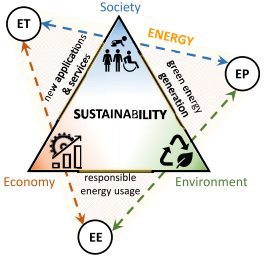
\includegraphics[width=0.5\textwidth]{img/005_SustainabilityTriangle.png}
        \caption{The Sustainability Triangle, highlighting the critical balance between environmental, social, and economic factors in achieving sustainable outcomes\cite{EnergySustainableIoT}.}
        \label{fig:sustainabilityTriangle}
    \end{figure}

\newpage
\subsection{Energy Efficiency}

    \paragraph{}
    \gls{energyEfficiency} is pivotal in reducing energy consumption and emissions. \gls{iot} devices enhance energy management across various sectors by enabling smart controls and predictive maintenance, while \gls{eh} technologies provide a sustainable energy supply by converting ambient energy into usable power.
    \begin{itemize}
        \item \textbf{\gls{iot}}: Enhances real-time energy monitoring and management, leading to significant energy savings and reduced waste\cite{HAFEZ2023101013}.
        \item \textbf{\gls{eh}}: Offers a renewable energy source, reducing reliance on traditional energy systems and enhancing device longevity\cite{LIU2023113436}.
    \end{itemize}

\subsection{Energy Resilience}

    \paragraph{}
    In the face of climate-induced disruptions, \gls{energyResilience} is increasingly critical. It involves the capacity of energy systems to withstand, adapt to, and recover from disturbances, ensuring stable and reliable energy supply\cite{iotSustainableEnergySystems}.
    \begin{itemize}
        \item \textbf{\gls{iot} for Resilience}: Employs real-time data and predictive analytics to enhance system responsiveness and recovery, contributing to a more distributed and less vulnerable energy infrastructure\cite{gameboyBatteryless}.
        \item \textbf{Energy Harvesting for Resilience}: Diversifies energy sources and enables autonomous operation, particularly beneficial in remote or disaster-prone areas, thus strengthening system robustness\cite{memsEHforIot}.
    \end{itemize}

\paragraph{}
The interconnectedness of \gls{sustainability}, \gls{energyEfficiency}, and \gls{energyResilience}, underpinned by \gls{iot}, \gls{mems} and \gls{eh} technologies, forms a cornerstone in the global response to climate change. Embracing these innovative approaches, as highlighted by the \gls{ipcc} and the UN's SDG reports, charts a path towards a sustainable, efficient, and resilient energy landscape. The collective pursuit of these objectives, in line with the urgent and inclusive climate action called for by these reports, is essential in mitigating climate impacts and securing a livable future for all.

Following the outlined context, we will delve into specific applications and the corresponding energy sources in the subsequent section.

\newpage
\subsection{Applications}

    \paragraph{}
    Below, we detail primary energy sources and their applications, as highlighted in \cite{greenIT} on page 8:
    \begin{itemize}
        \item \textbf{Motion} (\cite{eh_TorsionallyOscillatingMagnet}): This method encompasses \gls{electrostatic}, \gls{piezoelectric}, \gls{electromagnetic}, and \gls{magnetorestrictive} processes for powering IoT devices through movement. Its applications range from industrial uses, such as power transformers, to consumer technologies like battery-less gaming devices\cite{gameboyBatteryless}, vibration sensor in nuclear reactor\cite{iotSustainableEnergySystems}, to monitor and avert environmental radiation discharge.
        \item \textbf{Solar}: Utilizing light, \gls{photovoltaic} cells—both indoor and outdoor capable—serve as a versatile, renewable energy source crucial for infrastructure dependent on lighting schedules.
        \item \textbf{Thermal}: Exploiting temperature differentials allows for electricity generation useful in aerospace, automotive sensor enhancement, and wireless temperature management in food and pipelines, and for safety applications\cite{iotSustainableEnergySystems}.
        \item \textbf{Magnetic Field of Electric Power Lines}: Enhances electrical efficiency and transmission by harnessing naturally occurring magnetic fields.
        \item \textbf{Radio Frequency}: Key to \gls{rfid} technology, offering a sustainable alternative to standby modes in devices, conserving energy, and enabling early defect detection in maintenance.
        \item \textbf{Wind}: Facilitates environmental control in buildings through airflow energy harvesting.
    \end{itemize}

    \paragraph{}
    Additionally, beyond the succinct explanations provided for each energy source, numerous sectors will benefit significantly:
    \begin{itemize}
        \item \textbf{Healthcare}: Biometric wearables, harnessing motion energy, facilitate continuous health monitoring without battery dependence.
        \item \textbf{Maintenance Operations}: Energy sources across various sectors predict maintenance needs, adapt operations, and optimize consumption.
        \item \textbf{Military Operations}: \gls{terraswam} including \gls{smartdust}.
    \end{itemize}
    
    \paragraph{}
    These innovations not only enhance \gls{ee} but also contribute significantly toward our sustainability goals.
    

    \begin{figure}[htbp]
        \centering
        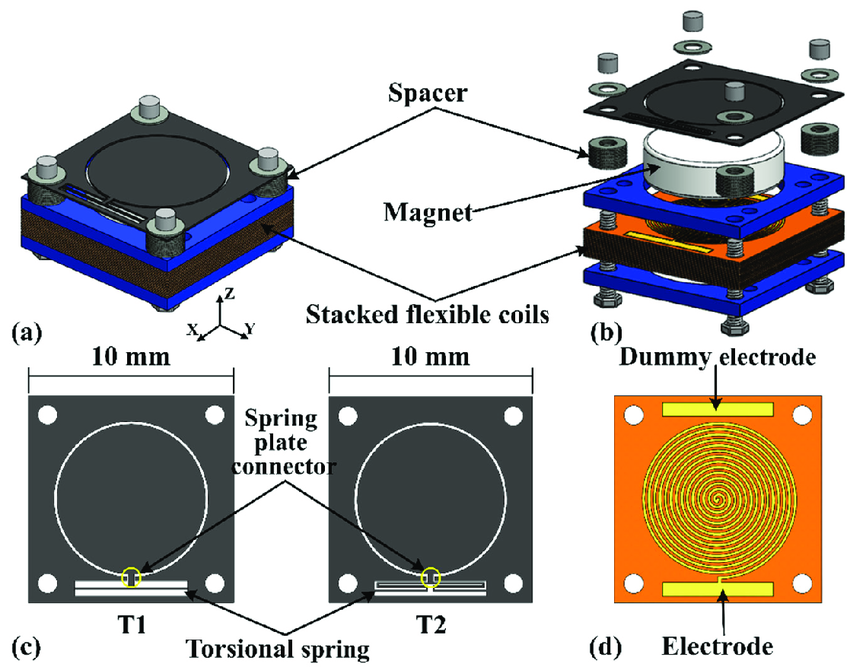
\includegraphics[width=0.5\textwidth]{img/006_EVEH.png}
        \caption{Schematic and exploded illustration of the assembled EVEH. (a) schematic illustration the \gls{eveh} device; (b) exploded view of the \gls{eveh} device; (c) two types of torsional spring; (d) layer of flexible coils\cite{eh_TorsionallyOscillatingMagnet}.}
        \label{fig:eveh}
    \end{figure} % Context

    \newpage
    \section{Primary Challenges}

    \paragraph{}
    In this section, we will highlight the challenges associated with the sustainability of \gls{eh} batteryless \gls{mems} and \gls{iot} devices.

    \subsection{Dynamic Power Management}

        \paragraph{}
        \gls{dpm} is crucial in the realm of ultra-low power IoT devices, focusing on optimizing device performance to align with workload demands, thereby reducing unnecessary power usage and enhancing energy efficiency. This strategy is increasingly important as the adoption of mobile and battery-dependent IoT devices grows, alongside the need for energy-saving operations in data centers and cloud computing. Efficient DPM practices\cite{powerMngtIoT} are key to meeting these challenges, emphasizing the significance of energy management in advancing the sustainability and effectiveness of IoT technologies.

        \paragraph{}
        The challenge of \gls{dpm} lies in developing algorithms and techniques that can dynamically adjust the power states of computing devices in response to changing workload demands, resource availability, and system conditions. Several factors contribute to the complexity of \gls{dpm}, including heterogeneous workloads, real-time constraints, and uncertain workload patterns\cite{10387280}.

        \paragraph{}
        Efficient \gls{dpm} strategies play a crucial role in improving energy efficiency, extending battery life, reducing operating costs, and minimizing environmental impact in computing systems. However, existing approaches to \gls{dpm} often suffer from limitations such as overhead and complexity, sensitivity to workload variability, and trade-offs between energy and performance.

        \paragraph{}
        Future research directions in \gls{dpm} include:
        \begin{itemize}
            \item The development of \gls{adaptivealg} (e.g.: \gls{rehash}),
            \item The \gls{selflearningalg},
            \item Integration of \gls{ml} \cite{SABOVIC2023100736}, and
            \item Exploration of novel hardware architectures.
        \end{itemize}

        \paragraph{}
        Addressing the challenge of \gls{dpm} requires interdisciplinary research efforts spanning computer science, electrical engineering, and materials science, with the potential to drive innovation and reshape the future of computing technology.
        

    \subsection{Low-Power Hardware Design}

        \paragraph{}
        In the realm of batteryless systems, \gls{lphd} plays a pivotal role in enabling energy-efficient operation without reliance on traditional power sources like batteries. This approach focuses on crafting hardware components, such as processors, memory modules, and sensors, that consume minimal power while delivering optimal performance. This is crucial for extending the lifespan and enhancing the efficiency of batteryless \gls{iot} devices\cite{ultraLowPowerIntegratedCircuitDesign}.

        \paragraph{}
        \gls{lphd} in batteryless systems entails the development of components capable of operating efficiently in energy-constrained environments. This involves minimizing the average power consumption during operation and standby modes, as well as ensuring compatibility with \gls{eh} mechanisms to utilize ambient energy sources effectively.

        \paragraph{}
        Despite advancements, \gls{lphd} in batteryless systems presents several challenges. One of the primary hurdles is achieving a balance between power efficiency and performance. Ensuring high performance while operating within strict power constraints necessitates innovative design approaches and meticulous optimization.

        \paragraph{}
        The complexity of \gls{lphd} for batteryless systems stems from various factors:
        \begin{itemize}
            \item \textbf{Energy Constraints}: Devices, especially those reliant on battery or ambient energy, have limited power resources. This necessitates hardware that can operate efficiently under such constraints.
            \item \textbf{Technological Limitations}: Existing hardware components are often designed for performance, with less emphasis on energy efficiency. Redesigning them for low power consumption without sacrificing performance is challenging.
            \item \textbf{Integration Issues}: Combining low-power components with traditional energy sources and ensuring they work seamlessly with other parts of the system can be complex.
            \item \textbf{Heat Generation}: High-power consumption leads to heat generation, which can damage components and affect device reliability and lifespan.
        \end{itemize}

        \paragraph{}
        To address the challenges of \gls{lphd} in batteryless systems, researchers and engineers have developed several strategies:
        \begin{itemize}
            \item \textbf{Ultra-Low-Power Components}: Development of components that utilize minimal energy for operation. This includes low-power processors, memory, and sensors.
            \item \textbf{Energy-Efficient Architectures}: Designing system architectures that minimize energy waste, including power gating and energy-efficient communication protocols.
            \item \textbf{Adaptive Power Management}: Implementing dynamic power management techniques that adjust the energy consumption based on workload, thereby optimizing the power use in real-time.
            \item \textbf{Use of Advanced Materials}: Exploring new materials and manufacturing techniques that can reduce energy consumption and remove toxic component\cite{ecofriendlyManufacturingiot}, such as using silicon on insulator (SOI) technology or carbon nanotubes.
        \end{itemize}

        \paragraph{}
        Despite progress, \gls{lphd} in batteryless systems still faces limitations:
        \begin{itemize}
            \item \textbf{Performance Trade-offs}: Achieving ultra-low power consumption often requires sacrificing some level of performance, which may not be acceptable for all applications.
            \item \textbf{Complexity and Cost}: Designing and manufacturing low-power hardware components can be more complex and costly than traditional components, potentially limiting their adoption.
            \item \textbf{Technological Barriers}: There are physical and technological limits to how much power efficiency can be improved, especially with current materials and technologies.
            \item \textbf{Compatibility and Integration Challenges}: Ensuring that low-power components integrate seamlessly with existing systems and technologies without compromising functionality can be difficult.
        \end{itemize}

        \paragraph{}
        \gls{lphd} is a multifaceted challenge with significant implications for the future of sustainable and energy-efficient electronics. While the responses to this challenge have been innovative and impactful, they come with inherent limitations that require ongoing research and development. Overcoming these limitations necessitates a holistic approach, incorporating advances in materials science, electrical engineering, and computer science to pave the way for the next generation of low-power devices.



    \subsection{Energy-Aware Software Design}

        \paragraph{}
        \gls{easd} is a critical aspect of modern computing, focusing on the development of software systems and applications that prioritize energy efficiency alongside performance and functionality. This approach aims to minimize energy consumption during software execution, thereby extending battery life, reducing energy costs, and mitigating environmental impact.

        \paragraph{}
        This encompasses the creation of algorithms, programming methodologies, and software architectures that optimize energy usage limit the sacrificing performance or user experience. It involves identifying energy-intensive tasks, optimizing resource utilization, and leveraging energy-saving techniques to maximize efficiency across various computing platforms\cite{basedArticle}, \cite{protean}.

        \paragraph{}
        Despite its importance, energy-aware software design poses several challenges. One of the primary obstacles is achieving a balance between energy efficiency and performance. Ensuring that software operates with minimal energy consumption while meeting performance requirements requires careful consideration of algorithmic complexity, resource utilization, and system dynamics\cite{9803046}.

        \paragraph{}
        The complexity of energy-aware software design arises from various factors:
        \begin{itemize}
            \item Diverse application domains: Software applications span a wide range of domains, each with unique energy requirements and constraints, making it challenging to develop generic energy-saving strategies.
            \item Heterogeneous hardware platforms: Software must run on diverse hardware architectures, including mobile devices, embedded systems, and cloud servers, each with different power characteristics and optimization opportunities.
            \item Dynamic workload patterns: Workload characteristics may vary dynamically, necessitating adaptive software designs capable of adjusting energy usage in real-time based on workload demands and system conditions.
        \end{itemize}

        \paragraph{}
        To address the challenges of energy-aware software design, researchers and practitioners have developed several strategies:
        \begin{itemize}
            \item Energy-efficient algorithms: Designing algorithms optimized for low energy consumption without compromising computational performance or accuracy.
            \item \gls{energyaware} programming models: Developing programming models and frameworks that abstract hardware details and provide \gls{poweraware} abstractions to application developers.
            \item Dynamic energy management techniques: Implementing runtime systems and middleware that monitor system energy usage and dynamically adjust software behavior to optimize energy efficiency.
        \end{itemize}

        \paragraph{}
        Despite advancements, energy-aware software design faces limitations:
        \begin{itemize}
            \item Trade-offs between energy and performance: Optimizing for energy efficiency may result in performance degradation or increased execution time, impacting user experience and application responsiveness\cite{EHandEE}.
            \item Complexity and overhead: Implementing energy-aware techniques may introduce additional complexity and computational overhead, potentially negating energy savings achieved by the software.
            \item Compatibility and portability: Energy-aware software designs may not always be compatible with existing systems or easily portable across different hardware platforms, hindering adoption and interoperability\cite{basedArticle}.
        \end{itemize}
        
        \paragraph{}
        The energy-aware software design is essential for building sustainable computing systems and applications. Overcoming the challenges and limitations through continued research, innovation, and interdisciplinary collaboration is crucial for realizing the full potential of energy-efficient software design and driving advancements in computing technology.



    \subsection{Energy Harvesting Integration}
    
        \paragraph{}
        \gls{eh} integration is a vital aspect of modern electronics, focusing on the seamless incorporation of \gls{eh} mechanisms into electronic systems to enable self-powered operation. This approach aims to utilize ambient energy sources, such as solar, kinetic, or thermal energy, to generate electricity for powering electronic devices and systems without the need for external power sources.

        \paragraph{}
        This involves the design and implementation of electronic systems and components capable of efficiently harvesting, storing, and managing energy from ambient sources. It encompasses the integration of \gls{eh} modules, power management circuits, and energy storage elements into electronic devices, enabling them to operate autonomously and sustainably in various environments\cite{EHandEE}.

        \paragraph{}
        Despite its potential benefits, \gls{eh} integration presents several challenges. One of the primary obstacles is maximizing energy extraction efficiency while ensuring compatibility with the target application's power requirements. Achieving optimal \gls{eh} performance across different environmental conditions and device configurations requires careful system design and optimization.

        \paragraph{}
        The complexity of \gls{eh} integration arises from various factors:
        \begin{itemize}
            \item Variability of ambient energy sources: Ambient energy sources, such as solar radiation or mechanical vibrations, exhibit variability in intensity, duration, and availability, posing challenges for consistent \gls{eh}.
            \item Energy storage and management: Efficiently storing and managing harvested energy requires sophisticated power management techniques and energy storage technologies capable of handling fluctuating energy inputs and varying power demands.
            \item Integration with existing systems: Retrofitting \gls{eh} capabilities into existing electronic systems or integrating them into new designs without compromising functionality or performance presents integration challenges.
        \end{itemize}

        \begin{figure}[htbp]
            \centering
            \includegraphics[width=0.9\textwidth]{img/003_EnergyHarvestingDevices.png}
            \caption{Diagram of a hybrid energy harvesting that uses both artificial and natural energies. \cite{jlpea13040062}, Page 3.}
            \label{fig:EnergyHarvestingDevices}
        \end{figure}

        \paragraph{}
        To address the challenges of \gls{eh} integration, researchers and engineers have developed several strategies:
        \begin{itemize}
            \item Adaptive \gls{eh} systems: Designing \gls{eh} systems equipped with adaptive algorithms and control mechanisms that optimize \gls{eh} performance based on environmental conditions and power requirements.
            \item Hybrid \gls{eh} approaches (figure \ref{fig:EnergyHarvestingDevices}, \cite{jlpea13040062}): Combining multiple \gls{eh} techniques, such as solar, kinetic, and thermal harvesting, to increase energy diversity and reliability and mitigate the limitations of individual harvesting methods.
            \item System-level optimization: Optimizing the overall system architecture, including \gls{eh} modules, power management circuits, and energy storage components, to maximize energy efficiency and system robustness.
        \end{itemize}

        \paragraph{}
        In summary, \gls{eh} integration holds great promise for enabling self-powered electronic systems and reducing reliance on external power sources. Overcoming the challenges and limitations through continued research, innovation, and collaboration is essential for realizing the full potential of \gls{eh} integration and driving advancements in sustainable electronics.
        


    \subsection{Adapting to Intermittent Energy Supply}

    \paragraph{}
    In the context of \gls{iot}, batteryless, and ultra-low power technologies, \gls{ies} refers to the challenge of ensuring continuous operation under conditions of fluctuating energy availability. This is particularly relevant for IoT devices deployed in remote or energy-constrained environments, where energy sources such as solar, ambient RF, or thermal gradients are subject to variability. The key is to harness these intermittent energy sources efficiently to power devices that require minimal energy for operation\cite{gameboyBatteryless}, \cite{basedArticle}.

    \paragraph{}
    The adaptation involves developing energy harvesting technologies and ultra-low power circuits that can operate in environments with highly variable energy inputs. Unlike traditional systems that rely on consistent power sources, IoT and ultra-low power devices must be designed to function effectively even with sporadic energy availability, leveraging the smallest amounts of energy for maximum utility\cite{EHandEE}.

    \paragraph{}
    The primary challenge in this domain is designing systems that are resilient to energy fluctuations, ensuring that IoT devices can maintain functionality without constant power supply. This includes optimizing energy storage, utilizing innovative batteryless technologies, and implementing power management strategies that adjust device operations based on available energy.

    \paragraph{}
    The complexity of adapting to \gls{ies} in IoT and ultra-low power systems involves several factors:
    \begin{itemize}
        \item Energy harvesting efficiency: Developing technologies capable of converting ambient energy sources into usable power with high efficiency, even under varying environmental conditions.
        \item Power management: Designing advanced power management circuits that minimize energy consumption and dynamically adjust device operations based on the current energy availability.
        \item Batteryless and energy storage solutions: Exploring innovative batteryless technologies and ultra-low power energy storage solutions that can provide reliable power supply despite intermittent energy generation.
    \end{itemize}

    \paragraph{}
    To address these challenges, various strategies have been developed:
    \begin{itemize}
        \item Adaptive energy harvesting: Implementing adaptive energy harvesting techniques that can optimize energy conversion from available sources in real-time, ensuring maximum power extraction.
        \item Ultra-low power design: Designing IoT devices and components that operate with minimal power consumption, extending operational life and reducing the need for frequent energy replenishment.
        \item Intelligent power management: Utilizing smart power management algorithms that dynamically balance energy harvesting, storage, and consumption to maintain continuous device operation.
    \end{itemize}

    \paragraph{}
    Despite advancements, adapting to \gls{ies} in the context of IoT, batteryless, and ultra-low power technologies poses several limitations:
    \begin{itemize}
        \item Operational constraints under low energy conditions: Ensuring reliable device functionality when energy availability is minimal remains a challenge.
        \item Energy storage and conversion efficiency: Improving the efficiency of energy storage and conversion mechanisms is critical for maximizing the utility of harvested energy.
        \item Integration and scalability: Integrating these technologies into a wide range of devices and applications, and scaling them to meet diverse operational requirements, presents ongoing challenges.
    \end{itemize}
    
    \paragraph{}
    Addressing the challenges of \gls{ies} in IoT, batteryless, and ultra-low power contexts requires innovative approaches that combine technological advancements, design optimization, and strategic power management. Overcoming these challenges is crucial for expanding the deployment of IoT devices in energy-constrained environments, paving the way for a more connected, efficient, and sustainable world.


    
    \subsection{Sensor Optimization}
    
        \paragraph{}
        Sensor optimization is a critical aspect of sensor design and deployment, focusing on enhancing the performance, efficiency, and reliability of sensors in various applications. This involves optimizing sensor parameters, configurations, and algorithms to achieve accurate and timely data acquisition while minimizing energy consumption and resource utilization.

        \paragraph{}
        Sensor optimization encompasses a range of techniques and strategies aimed at improving the effectiveness and efficiency of sensors. This includes optimizing sensor placement, calibration, sampling rates, and signal processing algorithms to maximize the quality and utility of sensor data while minimizing power consumption, latency, and cost\cite{ultraLowPowerIntegratedCircuitDesign}, \cite{EHandEE}.

        \paragraph{}
        The primary challenge of sensor optimization lies in achieving a balance between sensor performance and resource constraints. Designing sensors that deliver accurate and timely data while operating within limited power, memory, and processing resources requires careful optimization and trade-offs.

        \paragraph{}
        The complexity of sensor optimization arises from various factors:
        \begin{itemize}
            \item Resource constraints: Sensors deployed in resource-constrained environments, such as \gls{iot} devices or wireless sensor networks, must operate within strict limitations on power consumption, memory usage, and processing capabilities.
            \item Environmental variability: Environmental factors such as temperature, humidity, and interference can affect sensor performance and reliability, necessitating robust optimization techniques to mitigate their impact.
            \item Application-specific requirements: Sensors deployed in different applications, such as environmental monitoring, healthcare, or industrial automation, have unique requirements and constraints that must be considered during optimization.
        \end{itemize}

        \paragraph{}
        To address the challenges of sensor optimization, various strategies have been developed:
        \begin{itemize}
            \item Energy-efficient sensor design: Designing sensors with low-power components, optimized circuitry, and energy-efficient communication protocols to minimize power consumption and extend battery life.
            \item Adaptive sensing algorithms: Developing adaptive sensing algorithms that dynamically adjust sensor parameters and sampling rates based on environmental conditions, user requirements, and energy availability to optimize performance and efficiency.
            \item Distributed sensor networks: Deploying distributed sensor networks with decentralized processing and collaborative sensing capabilities to distribute computation and reduce energy consumption.
        \end{itemize}

        \paragraph{}
        Despite advancements, sensor optimization poses several limitations:
        \begin{itemize}
            \item Trade-offs between performance and resource consumption: Optimizing sensor performance may require increased power consumption, memory usage, or processing resources, leading to trade-offs that impact overall system efficiency and scalability.
            \item Sensing accuracy and reliability: Optimized sensor configurations and algorithms may sacrifice accuracy or reliability under certain conditions, affecting the quality and usefulness of sensor data.
            \item Complexity and implementation challenges: Implementing sophisticated optimization techniques and algorithms may introduce complexity and overhead, requiring specialized expertise and resources for design, development, and deployment.
        \end{itemize}

        \paragraph{}
       The sensor optimization is essential for maximizing the effectiveness and efficiency of sensor systems in various applications. Overcoming the challenges and limitations through continued research, innovation, and collaboration is crucial for realizing the full potential of sensor technology and enabling transformative applications in fields such as \gls{iot}, healthcare, environmental monitoring, and beyond.
        

    \paragraph{}
    In conclusion, addressing the sustainability of \gls{eh} batteryless \gls{iot} devices requires a multifaceted approach that tackles the challenges of \gls{dpm}, low-power hardware and software design, \gls{eh} integration, \gls{ies}, and sensor optimization. Overcoming these challenges necessitates ongoing research, innovation, and interdisciplinary collaboration to develop solutions that are not only energy-efficient but also practical, reliable, and scalable. % Primary Challenge

    \newpage
    \section{Other Challenges}

    \subsection{Energy-Efficient Communication Protocols}
    
        \paragraph{}
        The proliferation of \gls{iot} technology underscores the necessity for energy-efficient communication protocols crucial for the sustainability and operational longevity of \gls{iot} devices, especially in power-limited applications\cite{iotSustainableEnergySystems}.
        
        \paragraph{}
        The primary challenge stems from the inherent energy constraints of \gls{iot} devices and the need for constant data transmission.
        
        \paragraph{}
        Innovations include the development of \gls{lpwan} and advancements in protocols like \gls{coap} and \gls{mqtt-sn} designed to reduce power consumption\cite{SABOVIC2023100736}.
        
        \paragraph{}
        Challenges include maintaining high data transmission reliability while minimizing energy use and standardizing protocols across the \gls{iot} ecosystem.

    \subsection{Environmental Adaptability}
    
        \paragraph{}
        The effectiveness of \gls{iot} and energy harvesting technologies is influenced by their adaptability to environmental conditions\cite{iotSustainableEnergySystems}.
        
        \paragraph{}
        Environmental conditions can affect the efficiency of energy harvesters and device performance.
        
        \paragraph{}
        Efforts focus on creating resilient technologies adaptable to various conditions and integrating adaptive algorithms.
        
        \paragraph{}
        Main limitations include the complexity of designing adaptable devices without increasing costs or compromising efficiency.

    \subsection{Fault Tolerance}
    
        \paragraph{}
        The reliability of energy harvesting systems and \gls{iot} devices is critical, especially in remote or critical applications where maintenance is challenging. Fault tolerance—the ability to continue operation in the event of a component failure—is a key aspect of this reliability.
        
        \paragraph{}
        Variations in energy availability and environmental conditions can lead to unpredictable system behavior, while physical damage and component wear over time may also induce failures\cite{LIU2023113436}.
        
        \paragraph{}
        Techniques to enhance fault tolerance include redundancy, where critical components are duplicated to take over in case of failure, and the development of self-healing materials and circuits that can automatically repair minor damages.
        
        \paragraph{}
        Implementing fault tolerance increases the complexity and cost of devices. Moreover, there is a trade-off between the level of redundancy and the device's energy consumption and size.

    \subsection{Security and Privacy}
    
        \paragraph{}
        As \gls{iot} devices often collect and transmit sensitive data, ensuring their security and privacy is paramount. The challenge is magnified in energy harvesting \gls{iot} devices, where resource limitations may restrict the implementation of robust security measures.
        
        \paragraph{}
        The open and distributed nature of \gls{iot} networks, along with the use of standard communication protocols, can expose devices to various security threats, including data breaches and unauthorized access.
        
        \paragraph{}
        Developing lightweight cryptographic algorithms and secure communication protocols specifically designed for \gls{iot} environments. Efforts also include the use of blockchain technology to ensure data integrity and authentication\cite{iotSecurity}.
        
        \paragraph{}
        Achieving a balance between security level and energy consumption remains a significant challenge, as more sophisticated security measures typically require additional computational resources.

    \subsection{Lifecycle Management}
    
        \paragraph{}
        The environmental impact of \gls{iot} devices, particularly those enabled by energy harvesting technologies, extends beyond their operational life. Effective lifecycle management, including recycling and end-of-life disposal, is essential for minimizing this impact.
        
        \paragraph{}
        The increasing volume of electronic waste, coupled with the hazardous materials often used in electronic components, poses a significant environmental threat\cite{iotSustainableEnergySystems}.
        
        \paragraph{}
        Strategies include the design of devices with recyclable materials, the development of biodegradable electronic components, and the implementation of take-back programs for electronic waste.
        
        \paragraph{}
        The primary challenges are the cost and logistical complexity of recycling programs, as well as the current lack of standardization for the recyclability of \gls{iot} devices.
 % Secondary Challenge

    \newpage
    \section{Limitations}

        \paragraph{}
        The section effectively consolidates common limitations in the development and implementation of energy-efficient technologies and systems. It highlights five main areas: technological and economic challenges, performance trade-offs, infrastructure and policy constraints, integration challenges, and the complexity and cost of advanced techniques. Each point underscores critical barriers to scalability and adoption, pointing to the need for innovative solutions, supportive policies, and infrastructure improvements to overcome these hurdles and advance the sustainability of \gls{iot} and energy harvesting systems.



    \section{Potential Future Directions}

        \paragraph{}
        How can adaptive algorithms be designed and optimized to efficiently manage energy resources in \gls{iot} devices, taking into account factors such as energy availability, process priority, storage options, and operational frequency, to ensure the successful execution of processes?

        \paragraph{}
        This main question can be split into several sub questions:
        \begin{itemize}
            \item \textbf{Optimization in Ultra-Low Power Contexts}: In the context of ultra-low power, IoT, and battery-less environments, what strategies are most effective for designing and optimizing adaptive algorithms?
            \item \textbf{Decision-Making Based on Inputs}: How can an algorithm dynamically make optimal decisions to ensure successful process execution, considering varying inputs?
            \item \textbf{Algorithm Impact on System Resources}: How Algorithm can be adapted to different architectures (considering processor types, frequency, number of cores, etc.)?
            \item \textbf{System Resources influence Algorithm}: How the system resources (processor types, frequency, number of cores, ...) are impacting the adaptive algorithm?
            \item \textbf{Compiler Choice and Energy Consumption}: Does the choice of compiler have an impact on optimizing energy consumption, and if so, how?
            \item \textbf{Methodology Abstraction for Architectural Adaptability}: How can we improve the abstraction of adaptive algorithm methodologies to be applicable across different architectures?
            \item \textbf{"Rebound Effect" in Optimal Scheduling Algorithms}: What is the "Rebound Effect" resulting from the implementation of optimal scheduling algorithms, and how does it affect energy consumption?
            \item \textbf{Comparative Impact on Device vs. Core Consumption}: How does the adoption of adaptive algorithms affect the overall device consumption compared to core consumption specifically?
            \item \textbf{Application of \gls{process}, \gls{task}, and \gls{fsm}}: In the context of adaptive algorithms, how can processes, tasks, and FSMs be utilized effectively?
            \item \textbf{Completeness of Energy Complexity Theory}: Is the theory of energy complexity comprehensive enough to encompass the nuances of adaptive algorithm design in IoT devices?
        \end{itemize}



    \newpage
    \section{Conclusion}

        \paragraph{}
        This State of the Art unveils the intricate layers of sustainability in IoT ecosystems, particularly emphasizing the pivotal roles of Energy Harvesting, Efficiency, and Resilience.
        
        \paragraph{}
        By methodically dissecting the spectrum of challenges—from their genesis to current mitigative strategies and inherent limitations—this document lays a comprehensive foundation for understanding sustainability's multifaceted impact on IoT. Moreover, it critically evaluates these challenges, paving the way for future research through proposed thesis questions.
        
        \paragraph{}
        These inquiries, rooted in the document’s analytical insights, invite exploration beyond conventional boundaries, promising innovative solutions for a sustainable technological future.

    \newpage
    \appendix
\section{Methodology}
    
    \paragraph{}
    Our research delves into "Optimal scheduling for energy-harvesting batteryless sensory systems" highlighting key concepts like "Energy-Harvesting," "Batteryless," and "Scheduling." Our initial broad search scope was refined by incorporating terms such as "MEMS," "IoT," "Intermittent," and "Ultra Low Power" to closely align with our objectives of promoting "Energy Efficiency" and "Green IT."

    \paragraph{}
    Upon selecting publications based on relevance, citation count, and recency, we conducted further analysis by exploring additional works by the same authors and cross-verifying the gathered data to ensure accuracy.

    \paragraph{}
    This meticulous search strategy shaped our research framework, necessitating precise searches to enrich each section of our review. We predominantly sourced information from IEEExplorer, ACM Digital Library, ResearchGate, and Google Scholar, with selective contributions from DirectScience and Springer, to compile essential insights.

    
    			
    




    
    \newpage
    % Displaying the glossary at the end of the article and print it into ToC
    \printglossary[type=\acronymtype]
    \printglossary[type=main]

    \printbibliography[heading=bibintoc]

\end{document}